\subsection{Model}
We made a final class diagram based on class diagram on figure \ref{fig:pdaclassdiagram} -- from section \ref{sec:problem_structure} -- to show the design of the system with the MVC design pattern applied.
The new class diagram can be seen on figure \ref{fig:ClassDiagramV2}.


\begin{figure}%
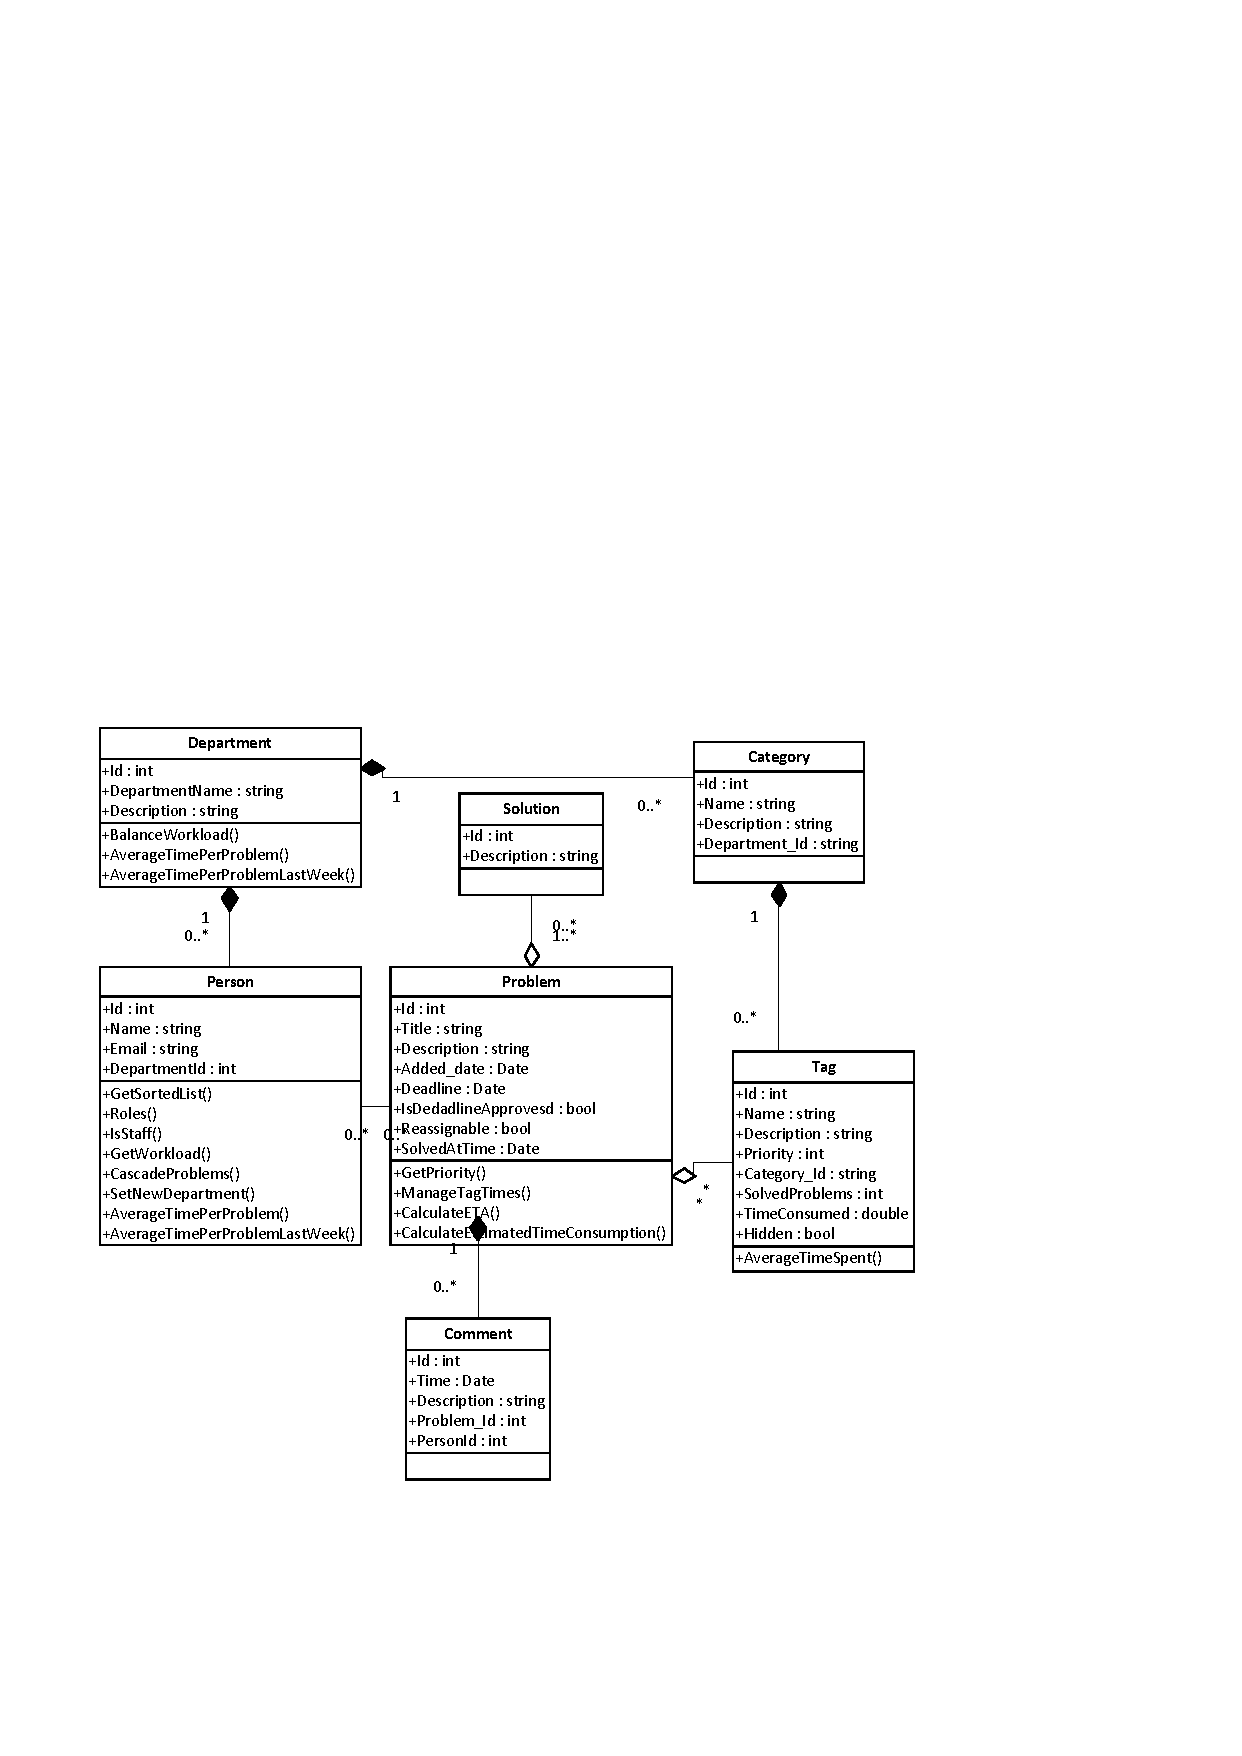
\includegraphics[width=\columnwidth]{input/component_design/ClassDiagramV2.pdf}%
\caption{The Class Diagram}%
\label{fig:ClassDiagramV2}%
\end{figure}


In the current design the following have been changed from the class diagram from section \ref{sec:problem_structure}:
\begin{itemize}	
	\item The role pattern: \\
	The functionality from the actor \admin[] does not inherit from \astaff[] and \aclient[] etc. Figure \ref{tab:newactortable} shows the new role system.   
	\item Problem: 
	\begin{itemize}
		\item \textbf{Deadline} \\
					The deadline is now a attribute instead of a class
		\item \textbf{Problem and tag relation} \\
					A tag can be connected to multiple different problems and a problem can have many tags connected to it. 
		\item \textbf{Problem and person relations} \\
					A person can have from zero to three simultaneous roles.				
	\end{itemize}
\end{itemize} 

\begin{figure}[p]
\begin{center}
\begin{tabular}{l  ccccc}
\hline 
\multicolumn{2}{r}{\shf{Actor}} \\
\shf{Use case} 	&   \Aclient 	& \Astaff 		& \admin[c]  \\ \hline%
Submit problem 	& $\checkmark$ 	&  	&  \\ %
My problems 		& $\checkmark$	&   &  \\ %
Worklist 				& 	& $\checkmark$  &  \\ %
Solve problem 	& 	& $\checkmark$	&  \\ %
Administrate		&  	&		& $\checkmark$ \\	%
\gstat[c]				&		& 	& $\checkmark$ \\ \hline%
\end{tabular}
\end{center}
\caption{\myCaption{Actor \& use case table}}
\label{tab:newactortable}
\end{figure}


\subsubsection{Description of Attributes for Each Class}

\begin{description}
\item[Problem]\hfill
\begin{description}
\item[Id:] A unique number which identifies each problem. 
\item[Title:] Contains the problems title.
\item[Description:] Contains the problems description.
\item[Added\_date:] The date and time of when the problem is added.
\item[Deadline:] A field where a date with a deadline can be added.
\item[IsDeadlineApproved:] Whether or not the problems deadline has been approved by the assigned \astaff[] member.
\item[Reassignable:] Whether or not a problem can be reassigned by the balance workload function \ref{sec:balanceworkload}. 
\item[SolvedAtTime:] If a problem has been solved, the time of completion is saved, if there is no SolvedAtTime then the problems status is unsolved.
\end{description}
\end{description}

\begin{description}
\item[Person]\hfill
\begin{description}
\item[Id:] A number which is unique for each Person. 
\item[Name:] The name of the person.
\item[Email:] The persons email, notifications are send to this email.  
\item[DepartmentId:] This the id of the persons department if any. 
\item[Other:] \fixme{skriv noget om aspnet person classen}
\end{description}
\end{description}

\begin{description}
\item[Department]\hfill
\begin{description}
\item[Id:] A number which is unique for each department. 
\item[DepartmentName:] The name of the department.
\item[Description:] Contains the description of the department.
\end{description}
\end{description}

\begin{description}
\item[Solution]\hfill
\begin{description}
\item[Id:] A number which is unique for each solution. 
\item[Description:] Contains the solution.
\end{description}
\end{description}

\begin{description}
\item[Category]\hfill
\begin{description}
\item[Id:] A number which is unique for each category. 
\item[Name:] The name of the category.
\item[Description:] Contains the description of the category.
\item[Department\_Id:] The id of the department which the category belongs to. 
\end{description}
\end{description}

\begin{description}
\item[Tag]\hfill
\begin{description}
\item[Id:] A number which is unique for each tag. 
\item[Name:] The name of the tag.
\item[Description:] The description of the tag.
\item[Priority:] Each tag have a weight, problems with high weight are prioritized higher.
\item[Category\_Id:] The id of the category which the tag belongs to. 
\item[SolvedProblems:] The number of problems which have been solved with this tag.
\item[TimeConsumed:] The total time problems with this tag have required to solve.
\item[Hidden:] Whether or not a tag is visible.
\end{description}
\end{description}

\begin{description}
\item[Comment]\hfill
\begin{description}
\item[Id:] A number which is unique for each comment. 
\item[Time:] The time and date when the comment is posted.  
\item[Description:] The content of the comment.
\item[Problem\_Id:] The id of the problem which the comment belongs to.
\item[PersonId:] The id of the person who wrote the comment.
\end{description}
\end{description}
